% !TeX root = ../main.tex

\chapter{附录}
\section*{一.信号采集系统}
本系统是用Labview语言编写的,使用前需要从NI官网上下载Labview程序以及NI-DAQmx驱动,操控的硬件设施为NI公司生产的“USB-6001”数据采集卡。
\subsection*{1.信号采集器}
本模块可以实时地采集四象限的Up-Down信号。使用步骤为:
\\1.打开“Casimir信号采集程序.vi”程序并运行,点击下拉列表,选择“信号采集器”;
\begin{figure}[h]
	\centering
	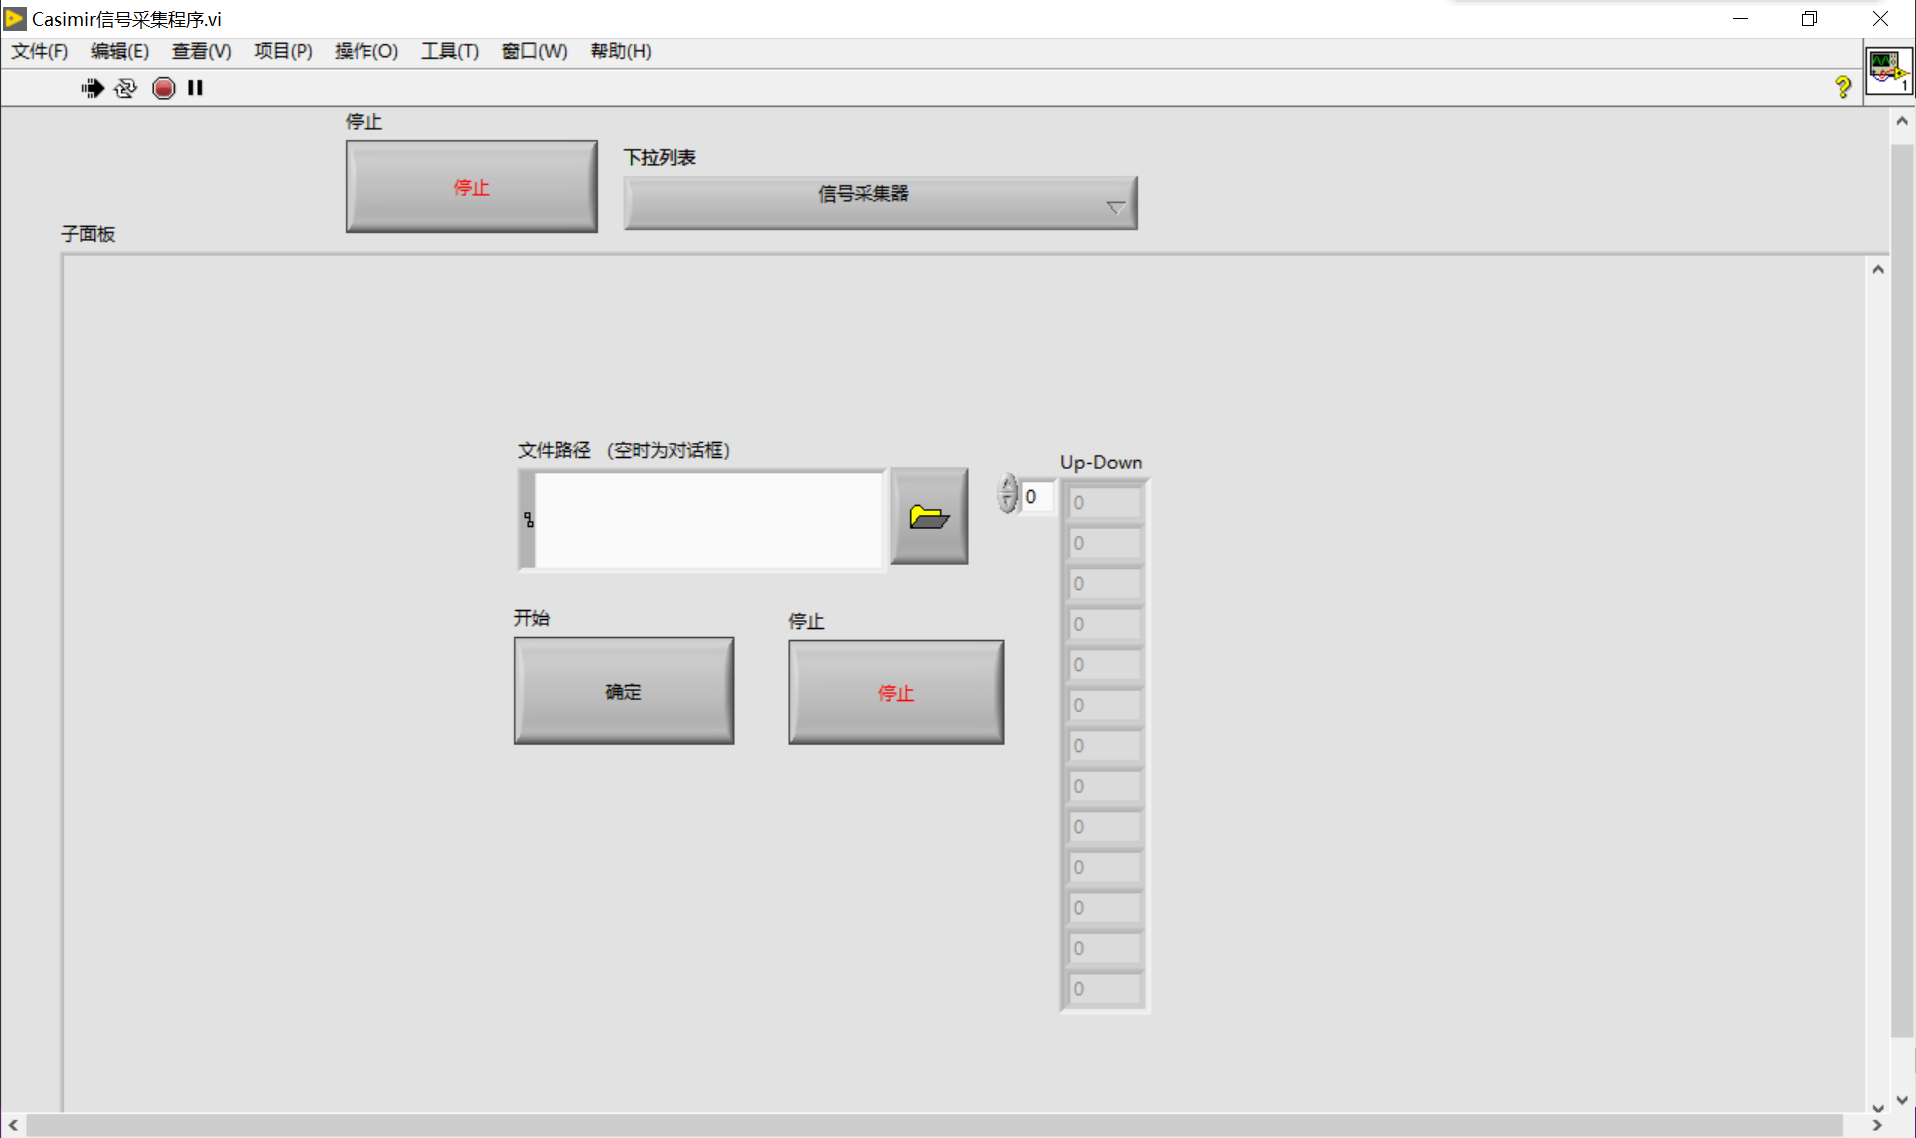
\includegraphics[scale=0.2]{信号采集器1}
	\caption{信号采集器}
\end{figure}
\\2.点击文件按钮选择需要存储信号的txt文档;
\\3.点击“开始”按钮开始采集信号,采集完成后点击“停止”按钮停止采集信号。
\subsection*{2.信号产生器}
本模块可以控制两个输出端口的电压信号。使用步骤为:
\\1.打开“Casimir信号采集程序.vi”程序并运行,点击下拉列表,选择“信号产生器”;
\begin{figure}[h]
	\centering
	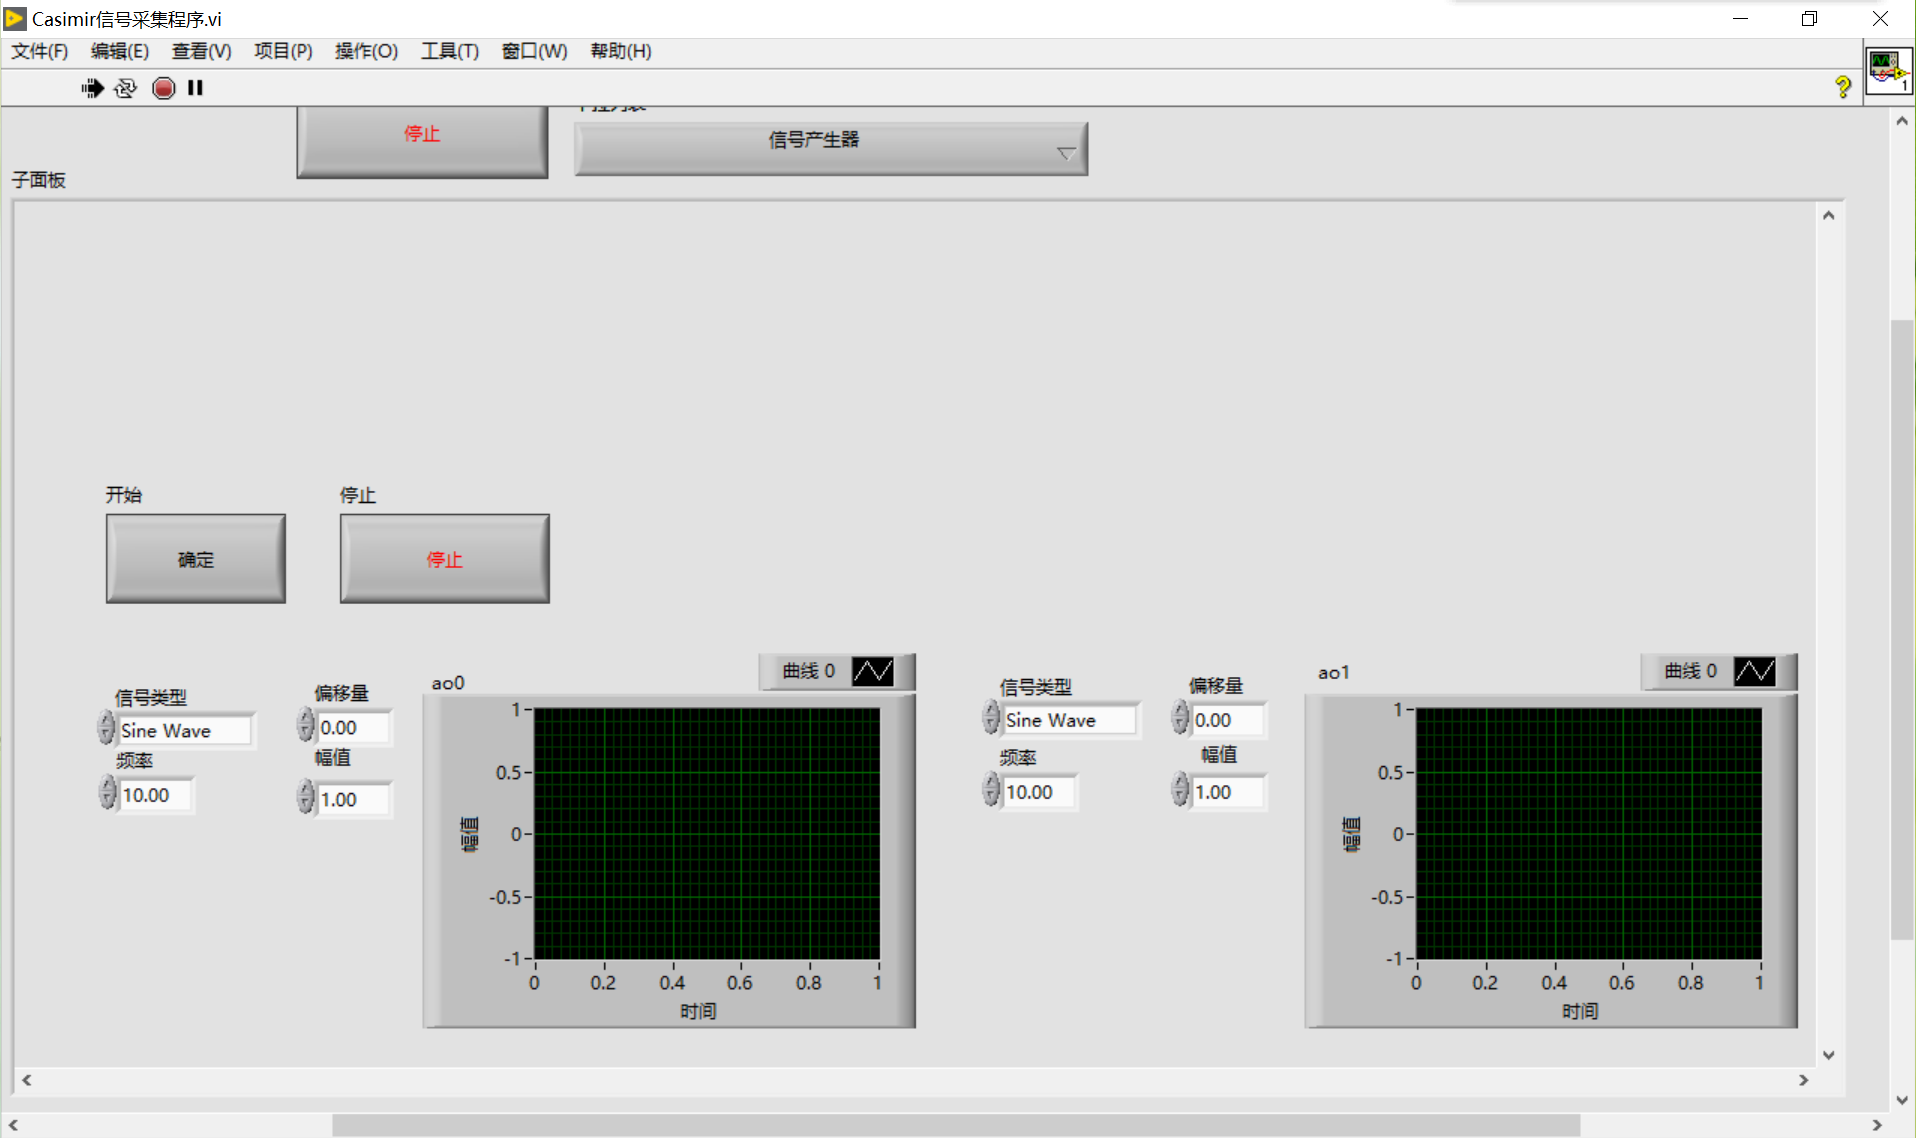
\includegraphics[scale=0.2]{信号产生器1}
	\caption{信号产生器}
\end{figure}
\\2.配置两个输出端口的电压信号参数,包括信号类型,偏移量,频率,幅值;
\\3.点击“开始”按钮开始输出电压信号,完成后点击“停止”按钮停止输出电压。
\newpage
\subsection*{3.探测样品的倾斜情况}
本模块可以测量样品沿某一方向的倾斜程度。使用步骤为:
\\1.打开“Casimir信号采集程序.vi”程序并运行,点击下拉列表,选择“探测样品的倾斜情况”;
\begin{figure}[h]
	\centering
	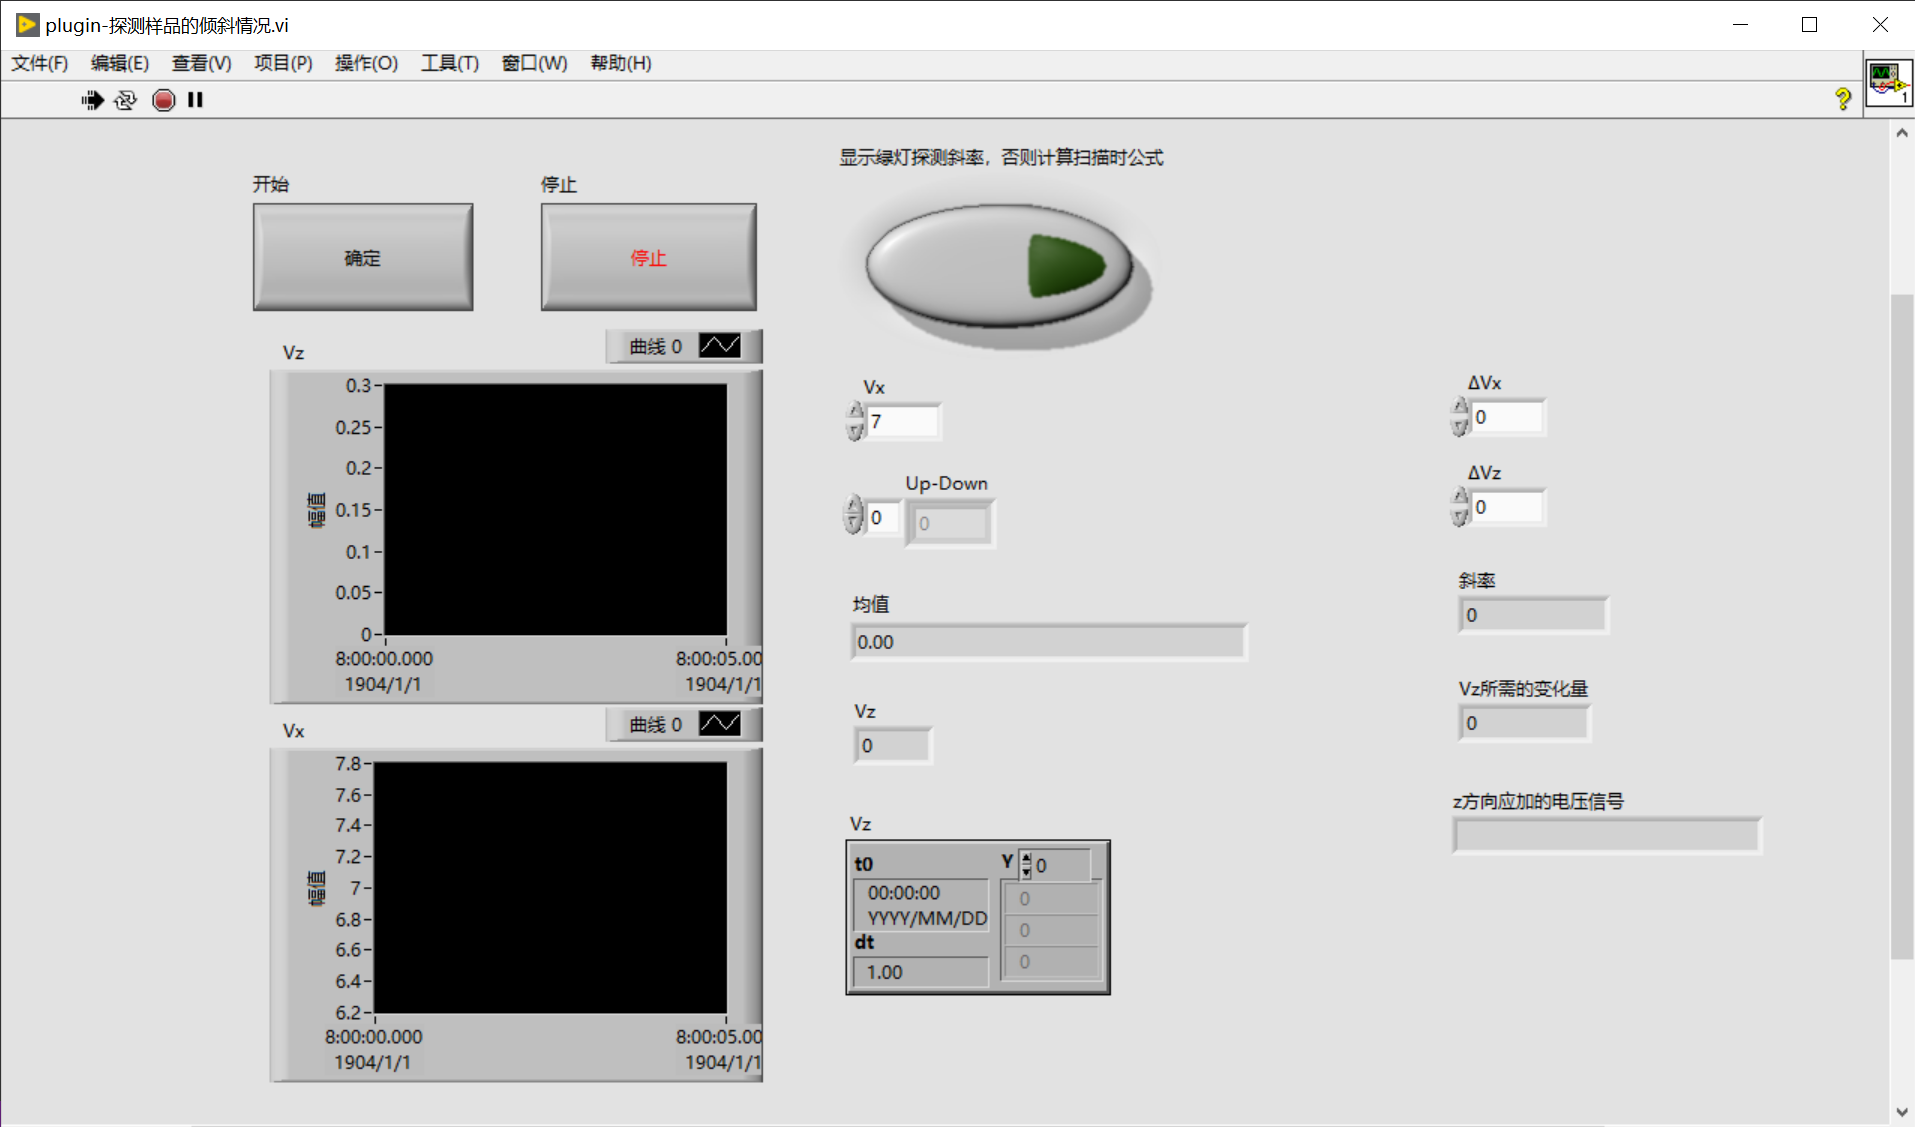
\includegraphics[scale=0.2]{探测样品的倾斜情况}
	\caption{探测样品的倾斜情况}
\end{figure}
\\2.点击上面的布尔开关使之处于打开的状态,设置Vx为8,点击“开始”按钮,观察左边Vz的波形图标,若Vz降到0V之前Up-Down均值一栏大于0.2,点击“停止”按钮,记录此时的Vz,然后再设置Vx为7,点击“开始”按钮,当Up-Down均值一栏大于0.2,点击停止按钮,记录此时的Vz,计算两次记录的Vz差值;若Vz降到0V之前Up-Down均值一栏一直小于0.2,设置Vx为-8,点击“开始”按钮,当Up-Down均值一栏大于0.2,点击停止按钮,记录此时的Vz,然后再设置Vx为-7,点击“开始”按钮,当Up-Down均值一栏大于0.2,点击“停止”按钮,记录此时的Vz,计算两次记录的Vz差值。
\\3.再点暗右上方的布尔按钮,输入$\Delta X$=1,$\Delta Z$ =两次记录的Vz差值,点击运行,得到扫描过程中Z方向应加的电压信号波形公式;
\subsection*{4.确定扫描的偏移量}
本模块可以确定扫描过程中应设置的z方向电压的偏移量。使用步骤为:
\\1.打开“Casimir信号采集程序.vi”程序并运行,点击下拉列表,选择“确定扫描的偏移量”;
\begin{figure}[h]
	\centering
	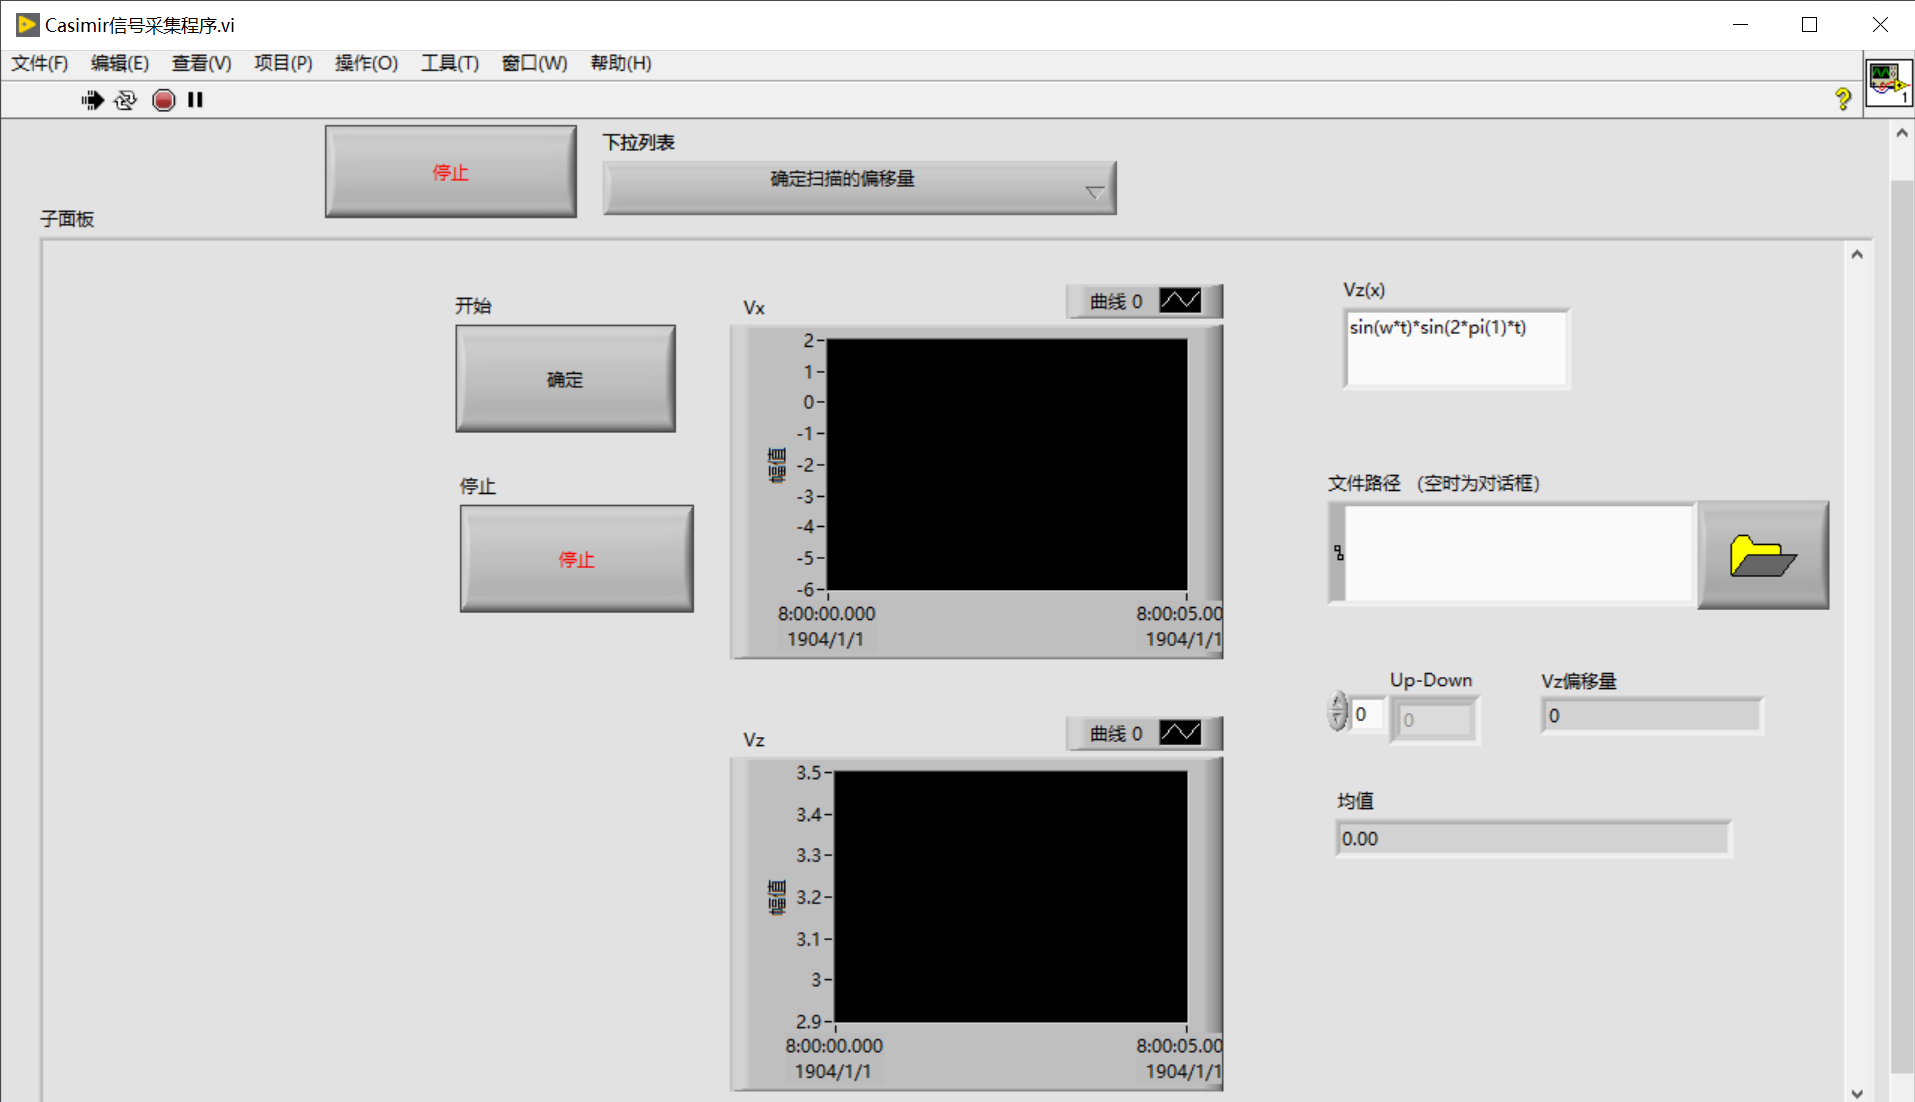
\includegraphics[scale=0.2]{确定扫描的偏移量}
	\caption{确定扫描的偏移量}
\end{figure}
\\2.前面板Vz(x)一栏应该填写由“探测样品的倾斜情况”程序计算出的“z方向应加的电压信号”,点击文件按钮,选择扫描过程中存储信号的txt文档;
\\3.点击“开始”按钮,等到"均值"一栏突变,点击“停止”按钮,记录"Vz偏移量"。
\subsection*{5.一维的扫描}
本模块可以一维地扫描样品并同时采集四象限信号值。使用步骤为:
\\1.打开“Casimir信号采集程序.vi”程序并运行,点击下拉列表,选择“一维的扫描”;
\begin{figure}[h]
	\centering
	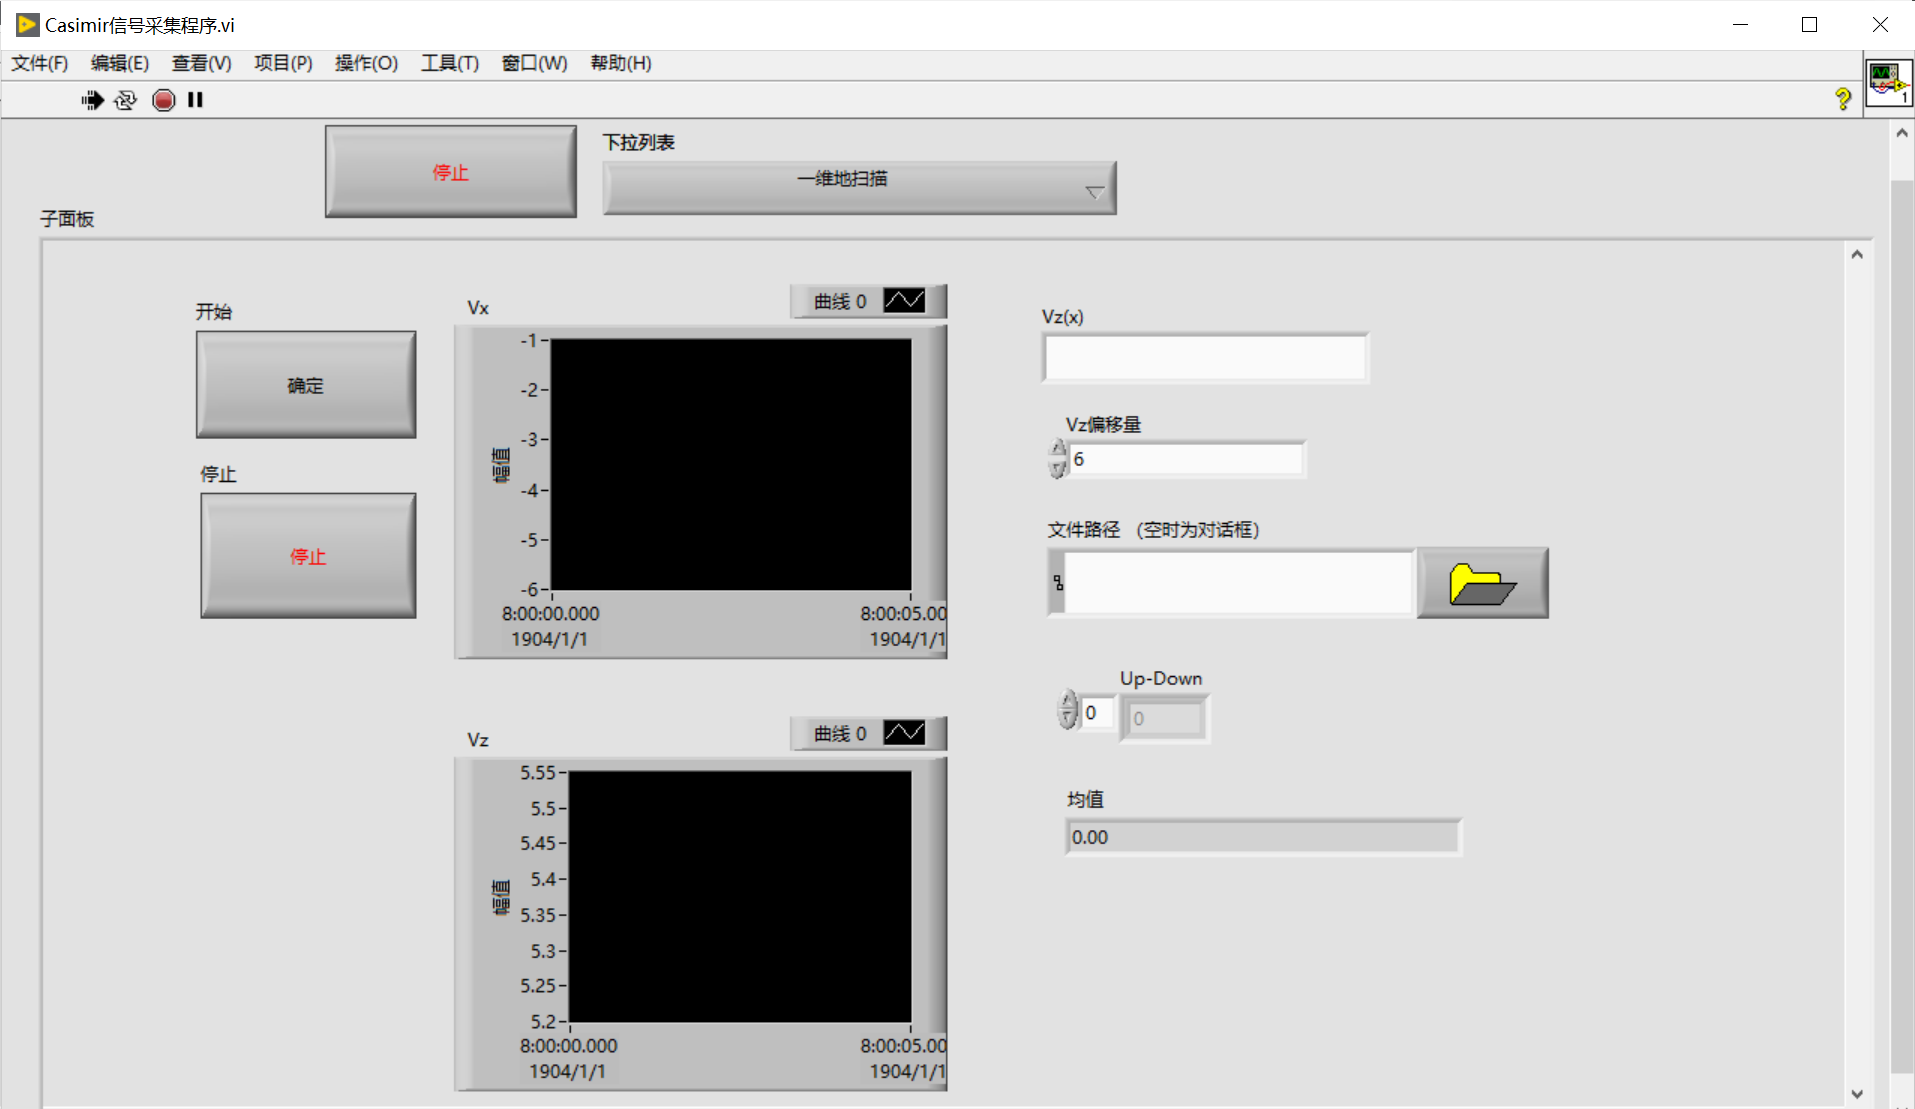
\includegraphics[scale=0.2]{一维地扫描}
	\caption{一维的扫描}
\end{figure}
\\2.前面板“Vz(x)”一栏应该填写由“探测样品的倾斜情况”程序计算出的“z方向应加的电压信号”,“Vz偏移量”一栏应该填写由“确定扫描的偏移量”程序测量到的“Vz偏移量”稍大的值(一般大0.05V就足够)。点击文件按钮,选择扫描过程中存储信号的txt文档;
\\3.点击“开始”按钮,等到扫描过程结束或者"均值"一栏突变,点击“停止”按钮。


\section*{二.信号处理系统}
本系统是用python语言编写的,使用前需要从python官网上下载python解释器。
\subsection*{1.做力曲线}
本模块可以处理仪器测量力曲线过程中“信号采集器”程序采集到的信号。使用步骤为:
\\1.打开“Casimir信号处理程序.py”,并运行程序;
\\2.选择“力曲线”功能模块;
\\3.输入设置参数,包括:Vz的最大值,最小值,压电陶瓷z方向的伸缩系数,探针劲度系数,去除跳变点个数,距离修正以及选择是否显示理论曲线;
\\4.点击导入文件按钮,导入采集到的txt文件;
\begin{figure}[h]
	\centering
	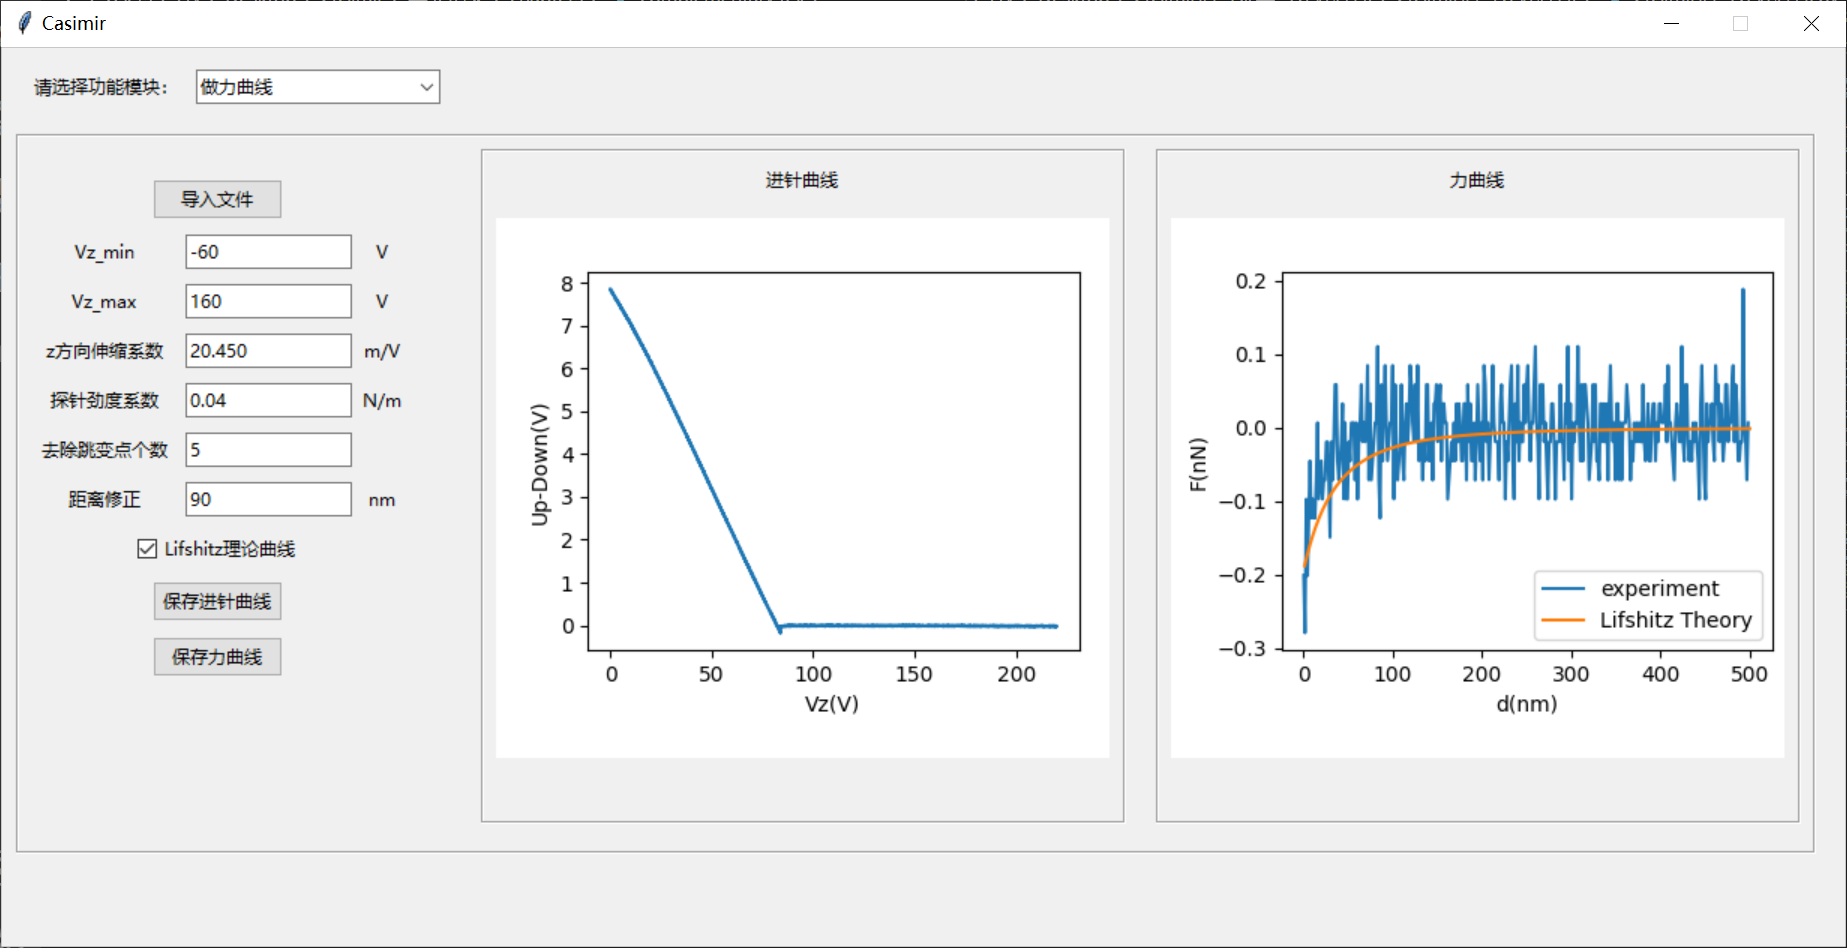
\includegraphics[scale=0.2]{做力曲线}
	\caption{做力曲线}
\end{figure}
\\5.点击保存图像按钮,保存对应的进针曲线或者力曲线图。
\subsection*{2.绘制扫描图像}
本模块可以处理一维或二维过程中采集到的信号。使用步骤为:
\\1.打开“Casimir信号处理程序.py”,并运行程序;
\\2.选择“绘制扫描图像”功能模块;
\\3.若要绘制一维扫描图案,点击“一维扫描”按钮,输入设置参数,包括:Vx的最大值,最小值,显示扫描的第几条曲线;点击导入文件按钮,导入采集到的txt文件;点击保存图像按钮,保存对应的一维扫描曲线。
\begin{figure}[h]
	\centering
	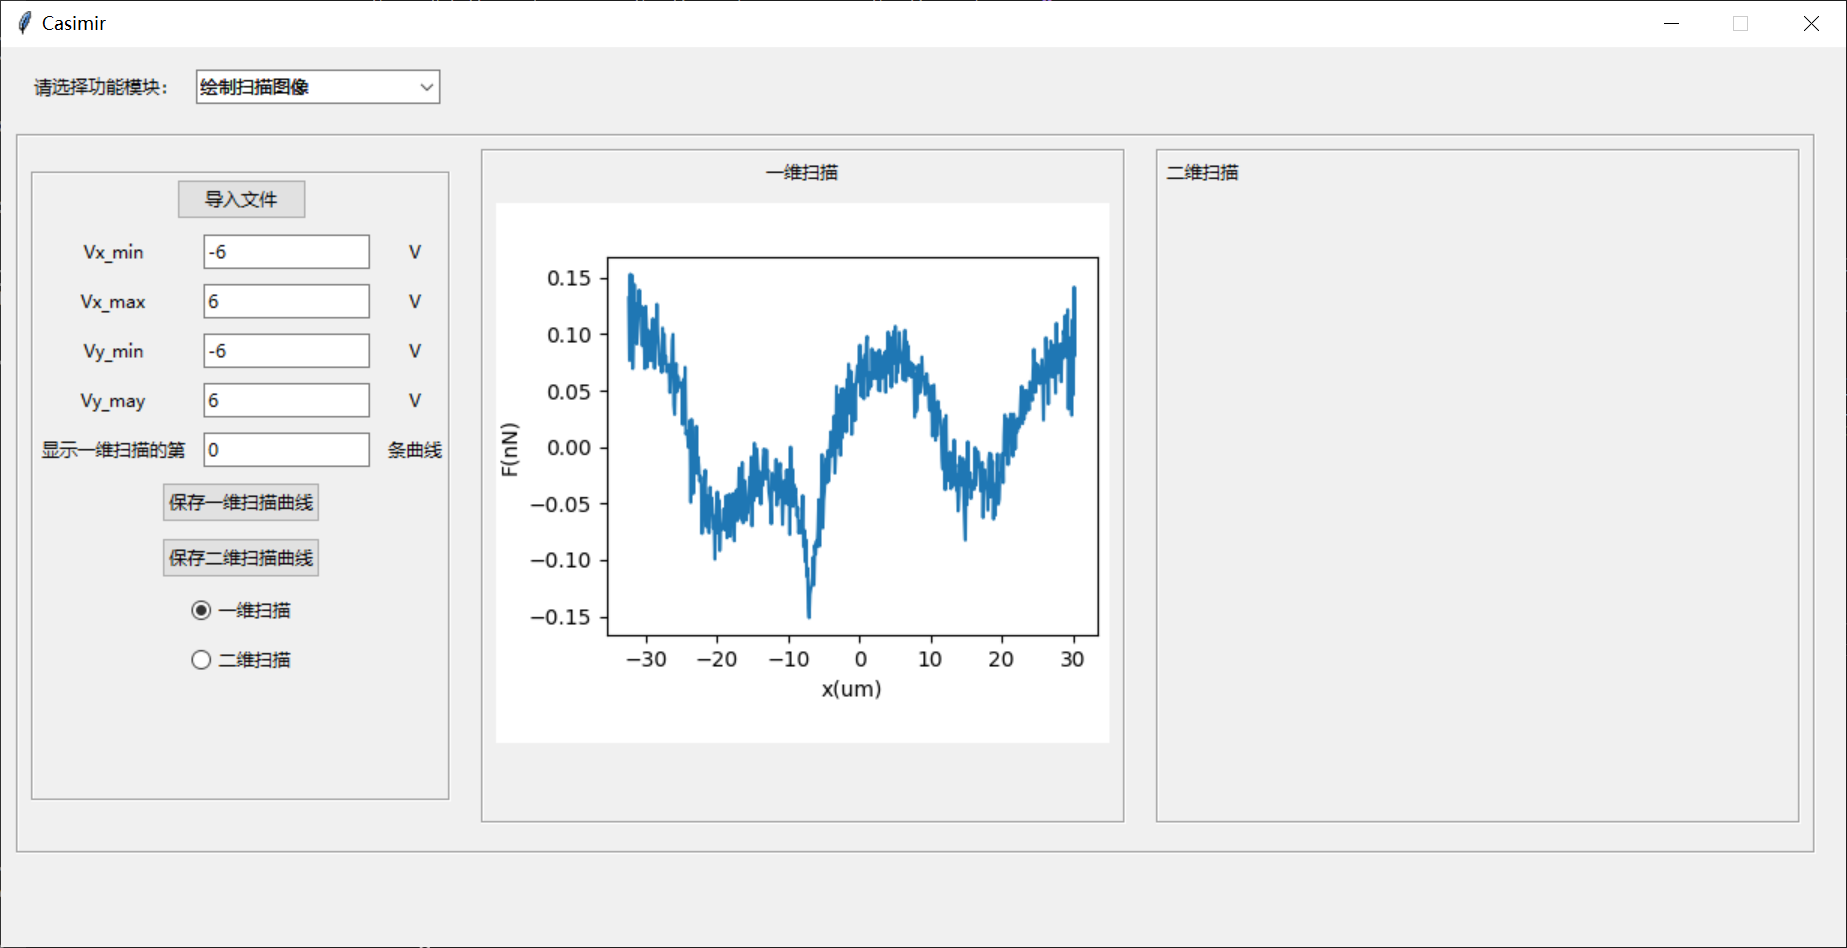
\includegraphics[scale=0.2]{一维扫描图}
	\caption{一维扫描图}
\end{figure}
4.若要绘制二维扫描图案,点击“二维扫描”按钮,输入设置参数,包括:Vx的最大值,最小值,Vy的最大值,最小值;点击导入文件按钮,导入采集到的txt文件;点击保存图像按钮,保存对应的二维扫描曲线。
\begin{figure}[h]
	\centering
	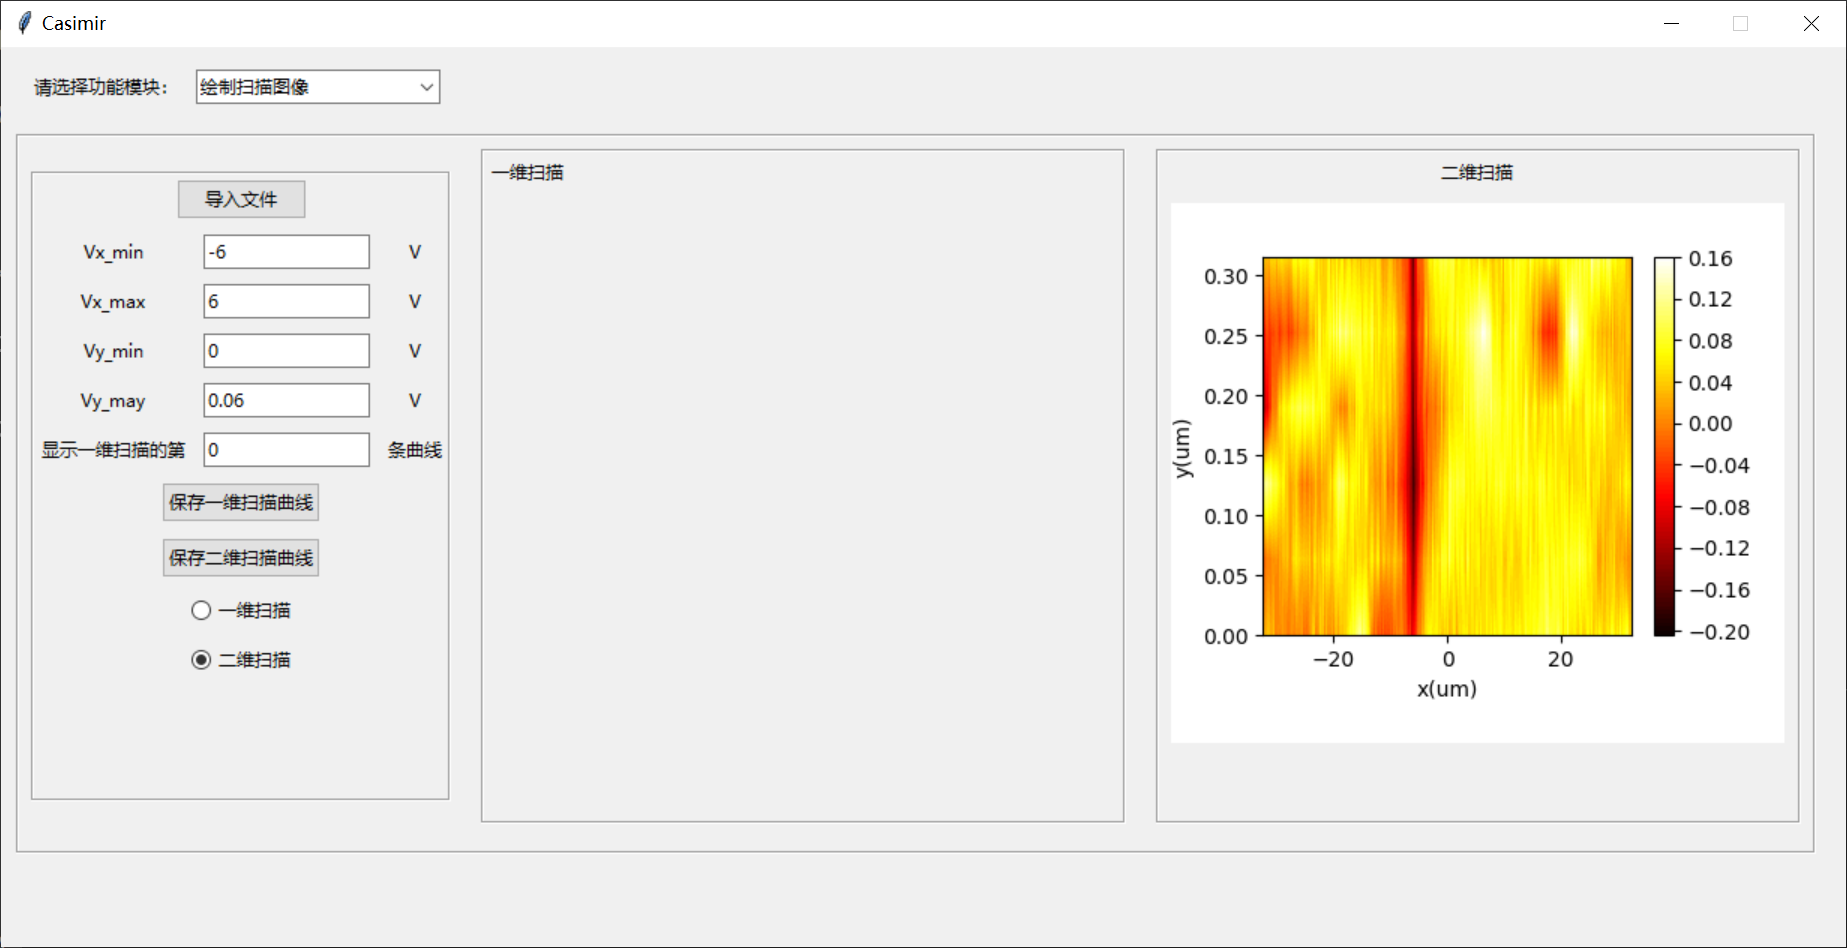
\includegraphics[scale=0.2]{二维扫描图}
	\caption{二维扫描图}
\end{figure}
